\documentclass{beamer}

\mode<presentation>
{
  \usetheme{default}      % or try Darmstadt, Madrid, Warsaw, ...
  \usecolortheme{default} % or try albatross, beaver, crane, ...
  \usefonttheme{default}  % or try serif, structurebold, ...
  \setbeamertemplate{navigation symbols}{}
  \setbeamertemplate{caption}[numbered]
}

\usepackage[english]{babel}
\usepackage[utf8x]{inputenc}
\usepackage{graphicx}    % Permite Gráficos
\usepackage{comment}
\usepackage{wasysym}

%%%\usepackage{wrapfig}




\title[Your Short Title]{ 
\includegraphics[scale=0.7]{logo_coca.jpg} \hspace{1cm}  COCA -- Applied Cognitive Computing Group}
\author{Grupo de Computação Cognitiva Aplicada -- COCA}
\institute{Computer Science Department -- UDESC}

\date{\today}

\begin{document}

%\begin{frame}
%\begin{figure}[h!]
%\begin{flushright}
% 
\includegraphics[scale=0.5]{logo_coca.jpg}
%\end{flushright}
%\end{figure}

 % \titlepage

%\end{frame}

\begin{frame}
\begin{columns}[T]

    \begin{column}{.6\textwidth}
     \begin{block}{}

 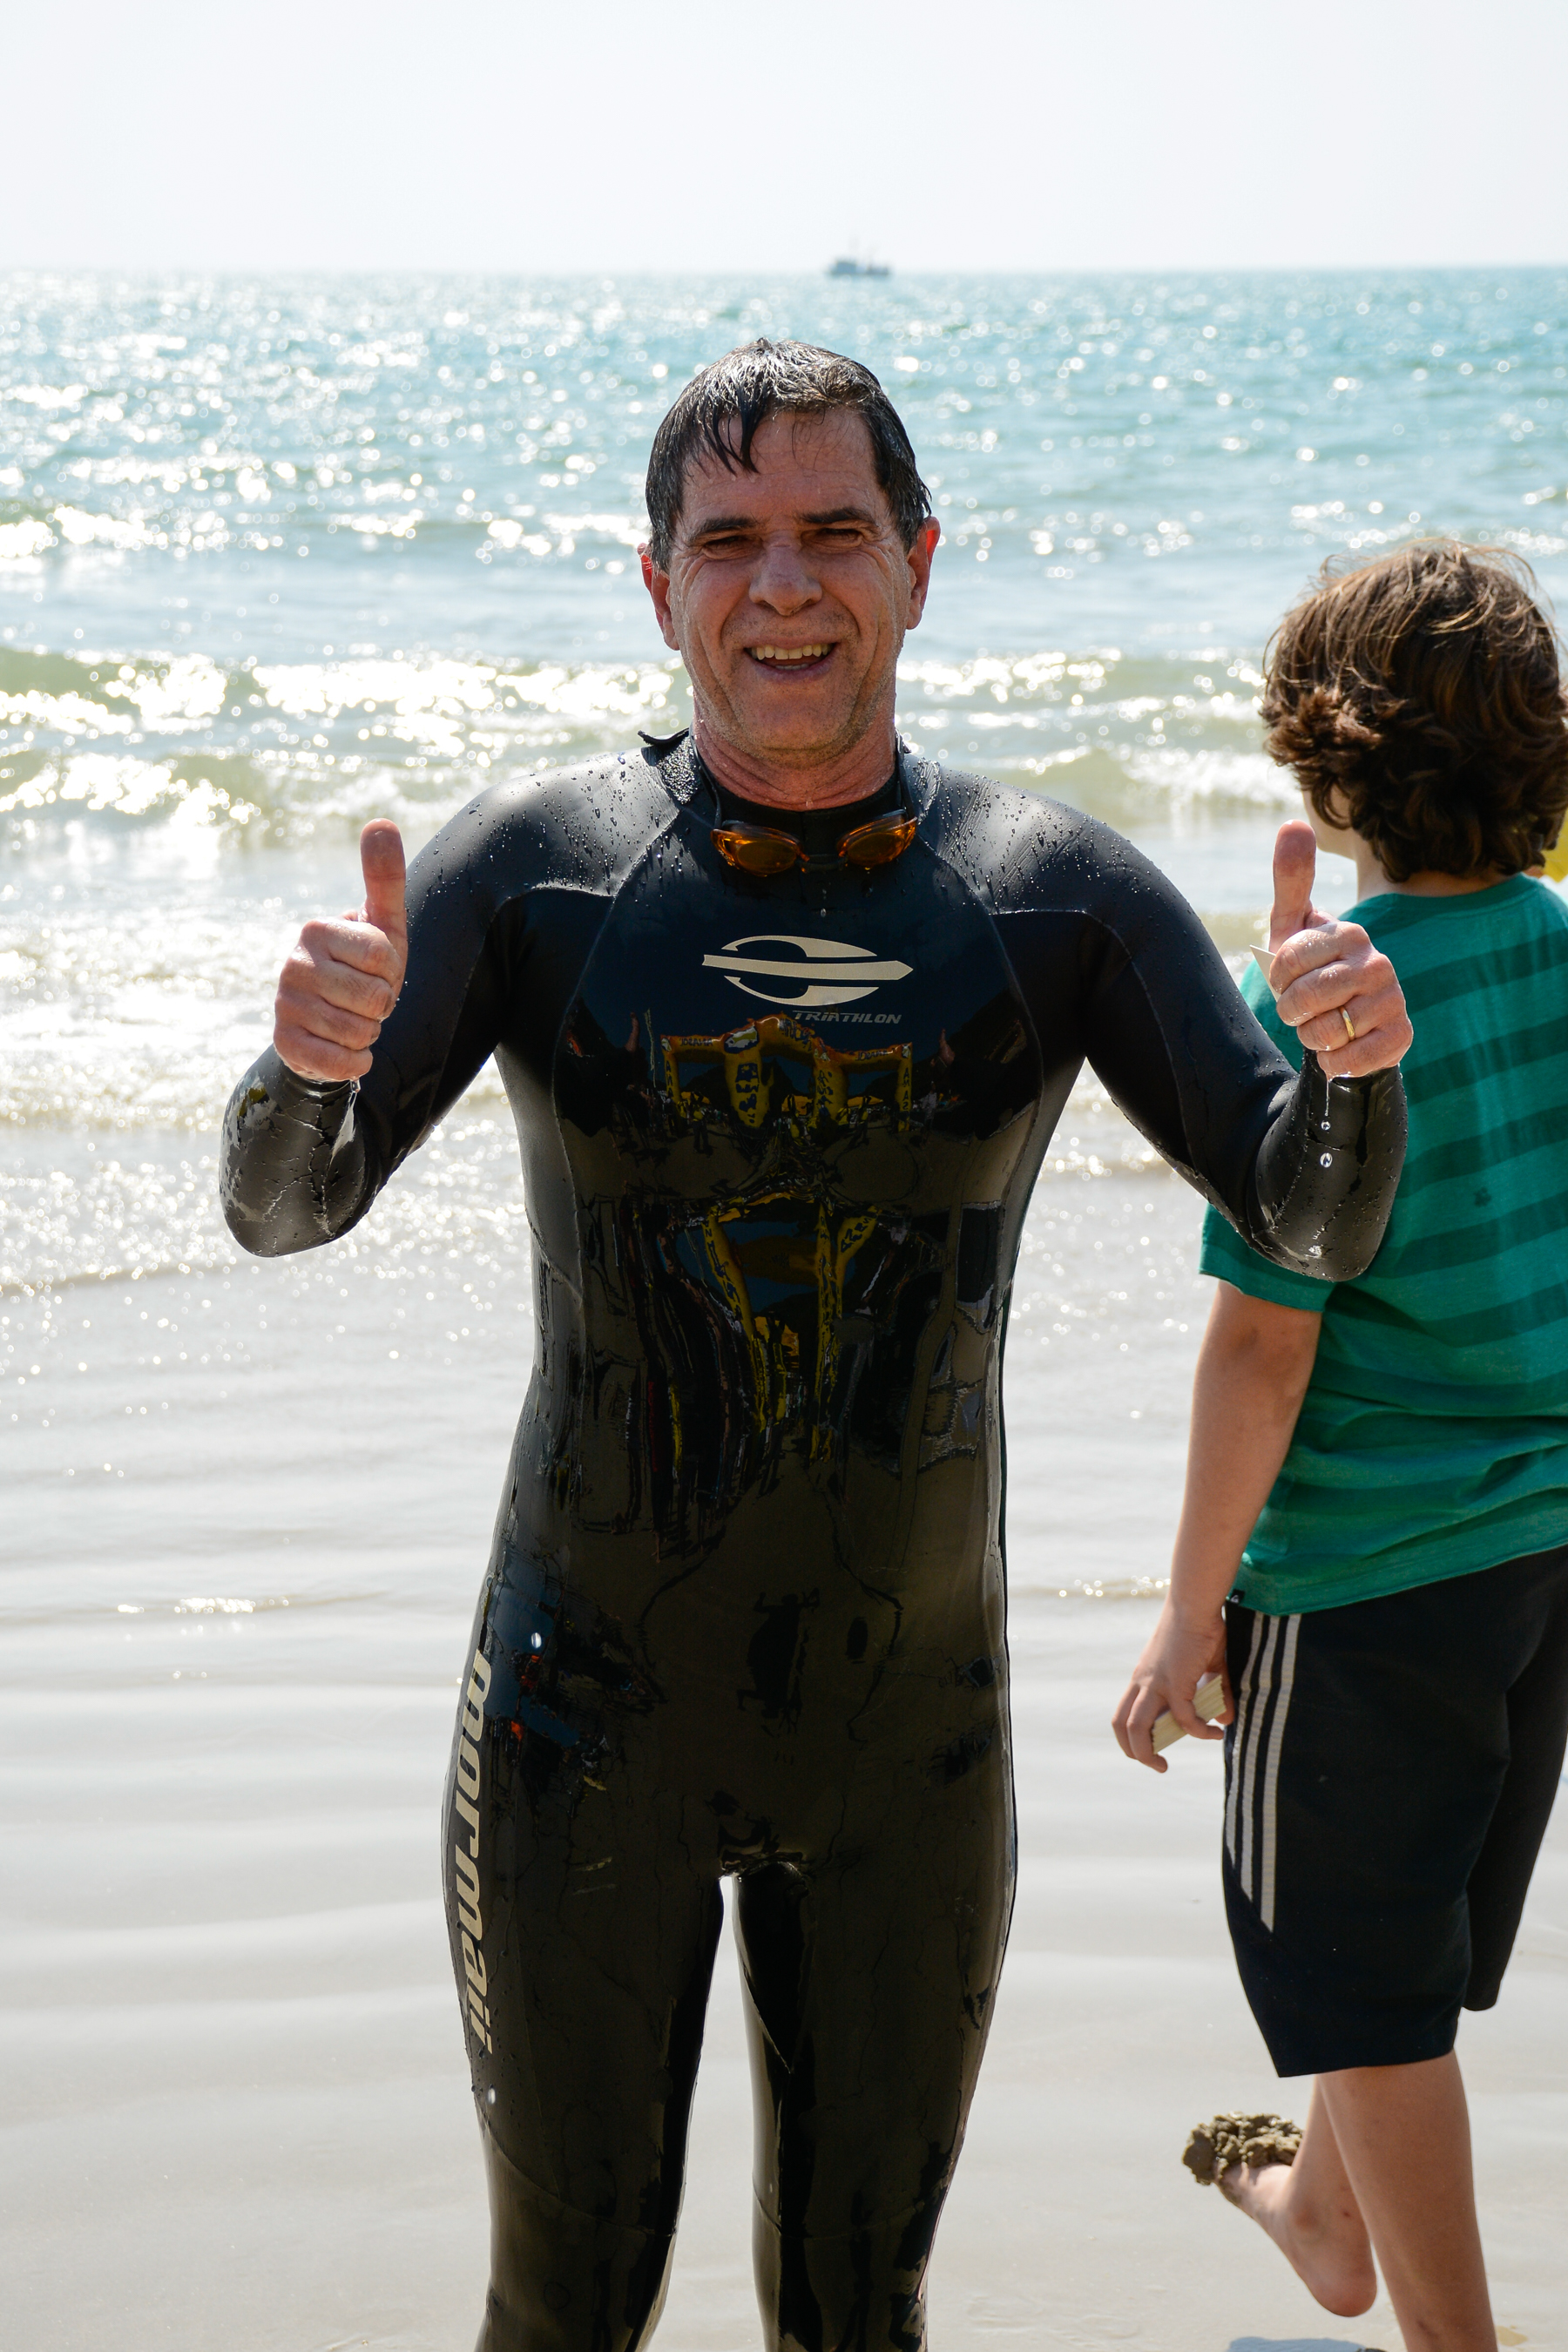
\includegraphics[scale=0.3]{figures/maratona01.jpg}
  
    \end{block}
    \end{column}
    \begin{column}{.5\textwidth}
    \begin{block}{}
    \vskip 2cm
    {\Large Claudio Cesar de Sá}\\
    {\large Independent Researcher in}\\
    {\large Computer Science}\\
     \today
    \end{block}
    \end{column}
  \end{columns}
\end{frame}





% Uncomment these lines for an automatically generated outline.
%\begin{frame}{Outline}
%  \tableofcontents
%\end{frame}


%%%%%%%%%%%%%%%%%%%%%%%%%%%%%%%%%%%%%%
\subsection{Claudio Cesar de Sá}

\begin{frame}{Claudio Cesar de Sá}

\begin{columns} %%% Começa o ambiente de Coluna
  \begin{column}{0.5\textwidth} %% 1a coluna
   \begin{itemize}
    \item Dr., Technological Institute of Aeronautics, 1997
    \item MSc., Master of Science in Electrical Enginering -- Federal University of Paraiba, 1987
    \item Graduate in Electrical Enginering -- State University of Santa Catarina, 1981
    \item ccs1664\{@gmail.com $\mid$ @yahoo.com\}
    \item Retired from UDESC since Noember--2019
    \end{itemize}
  \end{column}
   \begin{column}{0.6\textwidth}  %% 2a coluna --- SINGULAR
   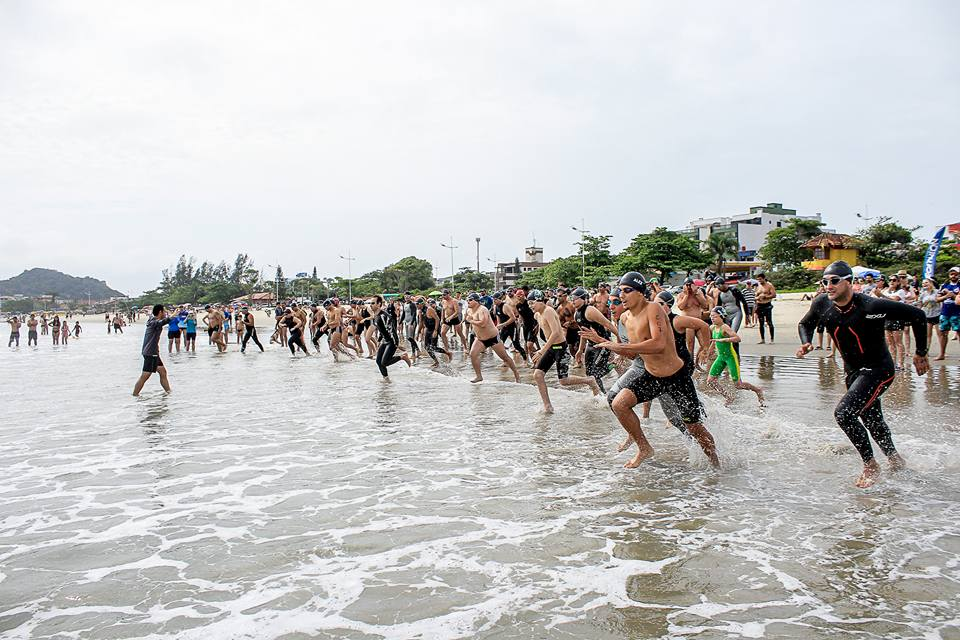
\includegraphics[scale=0.2,keepaspectratio]{figures/enseada01.jpg}
  \end{column} %%% SINGULAR
 \end{columns}
 
%%%%%%%%%%%%%%%%%%%%%% 
\end{frame}


\subsubsection{Computing}
\begin{frame}{Academic Activities}

\begin{itemize}
  \item Artificial Intelligence $\rightarrow $ applied to solve real problems
  \item Combinatorial (Discrete) Optimization
  \item Modelling with Constraint Programming
  \item Declarative Languages -- Haskell, Prolog and Picat
  \item Free Software Community
\end{itemize}

\end{frame}

\subsubsection{Teaching Duties}
\begin{frame}{Teaching Activities}

\begin{itemize}
  \item Mathematical Logic
  \item Theory of Computation
  \item Formal Methods
  \item Foundations of Constraint Programming
  \item Programming Languages
   \item Data Structures
\end{itemize}
\end{frame}

\subsubsection{Additional Activities}
\begin{frame}{Additional Activities}

\begin{itemize}
  \item Enrolled in Free Software Community
  \item General coordination: Contest Programming of ACM in UDESC
  \item Consulting of some enterprises: essentially courses
  \item Currently, aiming applications for free software and AI (models) for  {\em start-up} enterprises
\end{itemize}
\end{frame}

%%%%%%%%%%%%%%%%%%%%%%%%%%%%%%%%%%%%%%%%%%%%%%%%

\subsubsection{The Next Steps}
\begin{frame}{The Goals or Next Steps:}
\label{next_steps}
\begin{itemize}
  \item Some invitations to write books 
  \item The usage of Picat in planning applied  ...
  \item A language for model description  in Haskell 
  \item The Minizinc codes for description of models (other direction)
  \item Some AI tools applied in  {\em start-up} enterprises
  \item Hybridization of discrete techniques, such CP for instance, 
    and an evolutionary approach
\end{itemize}
\end{frame}

%%%%%%%%%%%%%%%%%%%%%%%%%%%%%%%%%%%%%%%%%%%%%%%%%%%%%%%%%%%%%%%%%%%%%%%%%%%%%%%%%%%%%%%%%%%%%%%%

%%%%%%%%%%%%%%%%%%%%%%%%%%%%%%%%%%%%%%%%%%%%%%%%


\end{document}
